この章では低温にした際, 懸架装置の特性がどのように変化するかということについて述べる. 
\section{特性評価の目的}
第\ref{第1章}章で述べた通りKAGRAでは鏡を極低温に冷却するが, これは2023年現在運転中の他の重力波検出器にはない大きな特徴である. しかし, 低温にすると鏡や懸架ワイヤなどの物性が変化することで共振周波数や伝達関数も変化する. すると, それに伴いかけるべき制御も変更する必要が生まれることがある. そこで低温にした際, ローカル制御に用いるフォトセンサの出力や懸架装置の伝達関数, Q値が室温と比較してどのように変化したかを調べた. \\
\quad なお, ETMY, ITMX, ITMYは2022年1月現在$250$ Kほどまでしか冷却されていないため, ETMXについてのみ, 特性評価を行った. \\
\quad また,  ETMXのMNの温度変化は図\ref{fig5.1}の通りであり, 277 Kから82 Kまで冷却された状態で特性評価を行った. 
\begin{figure}[H]
\begin{center}
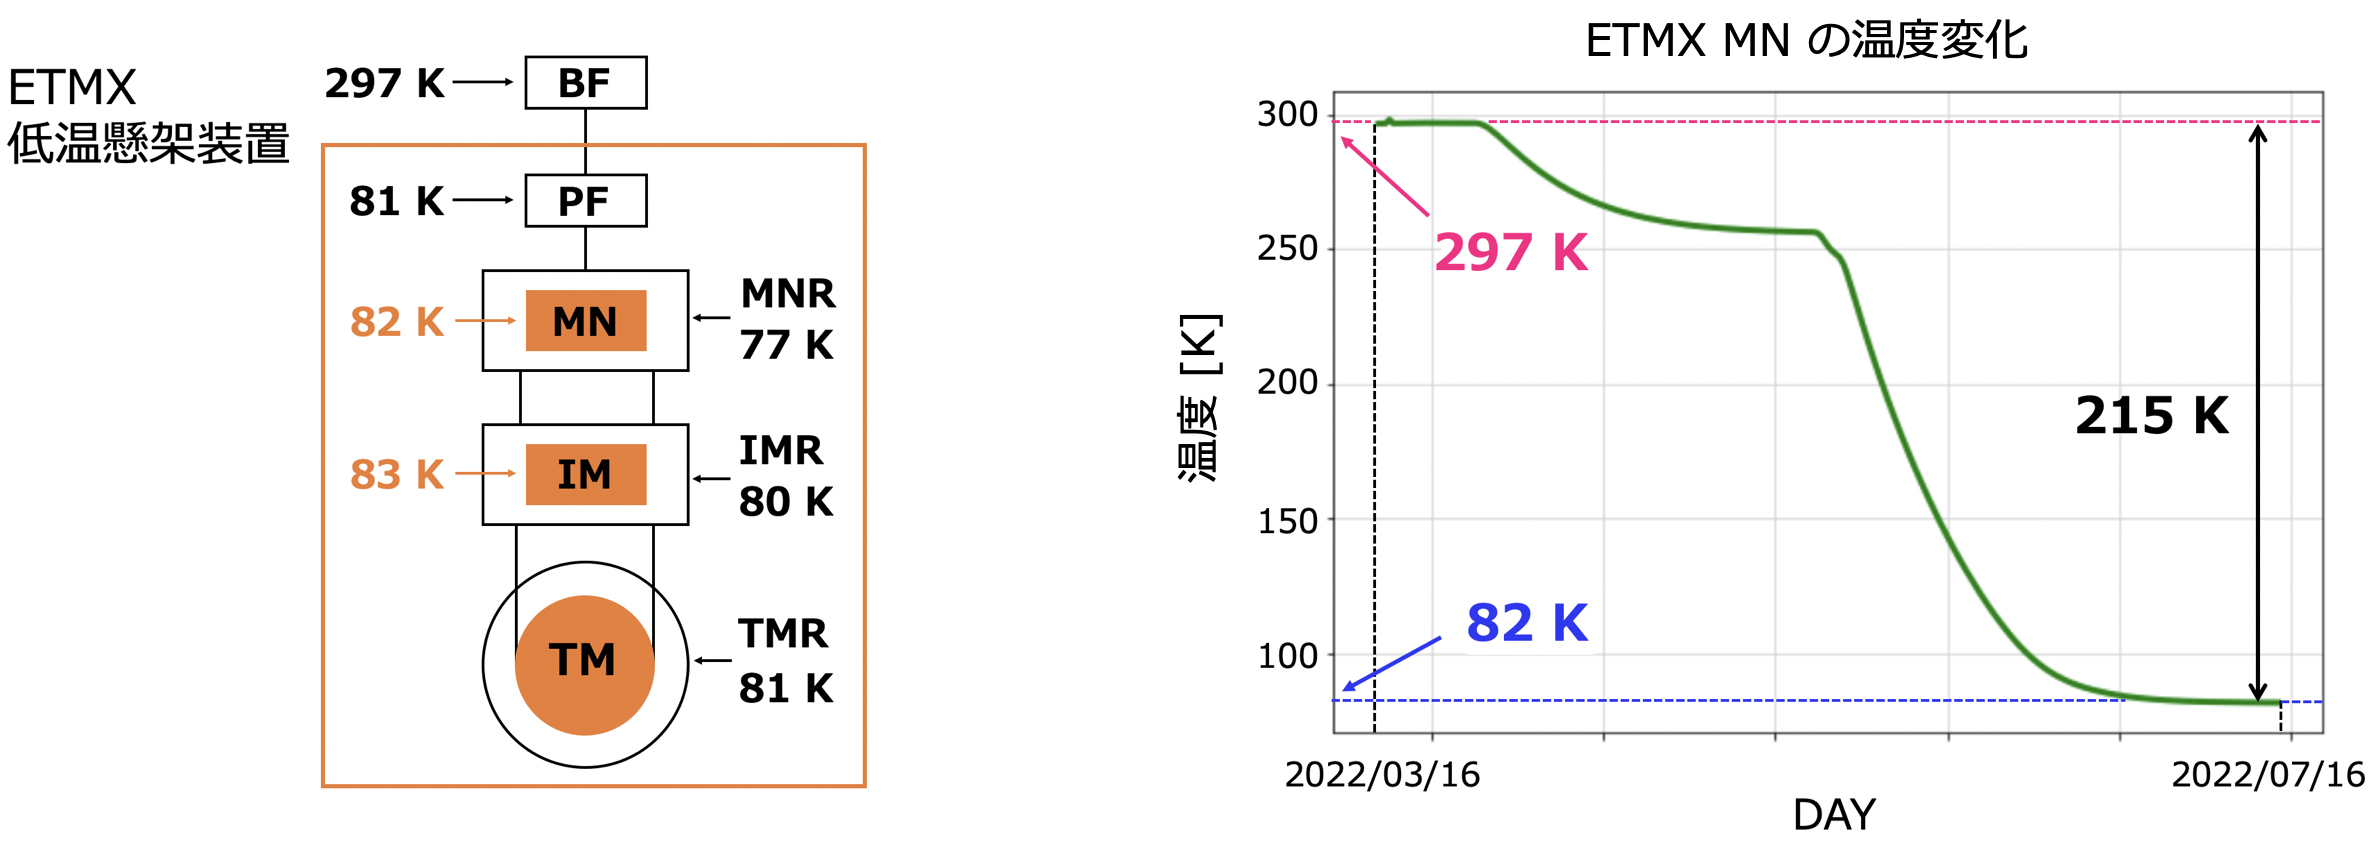
\includegraphics[width=170mm]{fig5_1.png}
\caption[ETMXの低温懸架装置の温度]{ETMXの低温懸架装置の温度(左)とETMX MNの温度変化(右)}
\label{fig5.1}
\end{center}
\end{figure}
\section{室温と低温下での特性の比較}
\subsection{フォトセンサの出力}
第4章で述べたように, 反射型のフォトセンサを用いてMN, IM段とそれぞれのリコイルマスとの距離を測定し, その信号を用いてローカルな制御を行っている.  ここではフォトセンサの出力が室温から低温への変化でどのように変化するか調べた. 
\subsubsection{測定結果}
\vskip3mm
MN, IM段で用いられるフォトセンサの出力を室温と低温下で比較したところ, 図\ref{fig5.2}, \ref{fig5.3}のようになった. これらの図では室温 (297 K) での出力を1とし, 他の温度ではそれに対して何倍の出力があるかということを示した. \\
\quad これより, 低温にするとフォトセンサの出力が増加するのが分かる. これは, 低温にすると小さな変化をより大きく見られることを示しており, またインストール前に\cite{47}で測定された結果と一致している.  \\\\
\begin{figure}[H]
\begin{center}
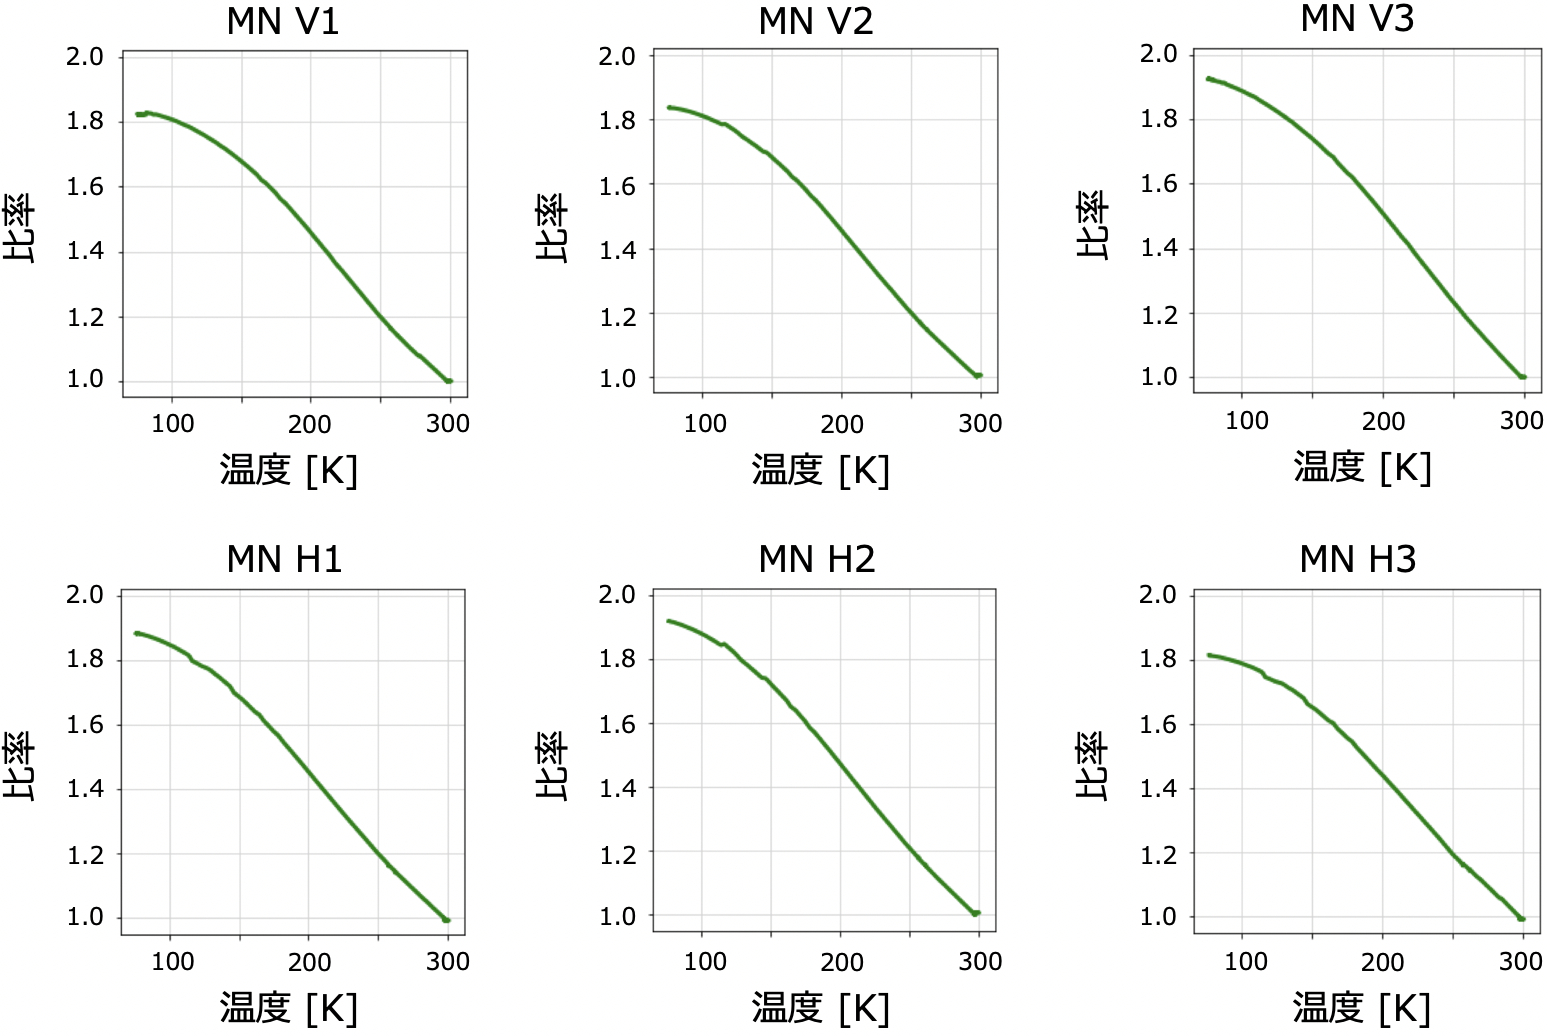
\includegraphics[width=160mm]{fig5_2.png}
\caption[フォトセンサの出力(ETMX MN)の変化]{フォトセンサの出力(ETMX MN)の変化}
\label{fig5.2}
\end{center}
\end{figure}
\begin{figure}[H]
\begin{center}
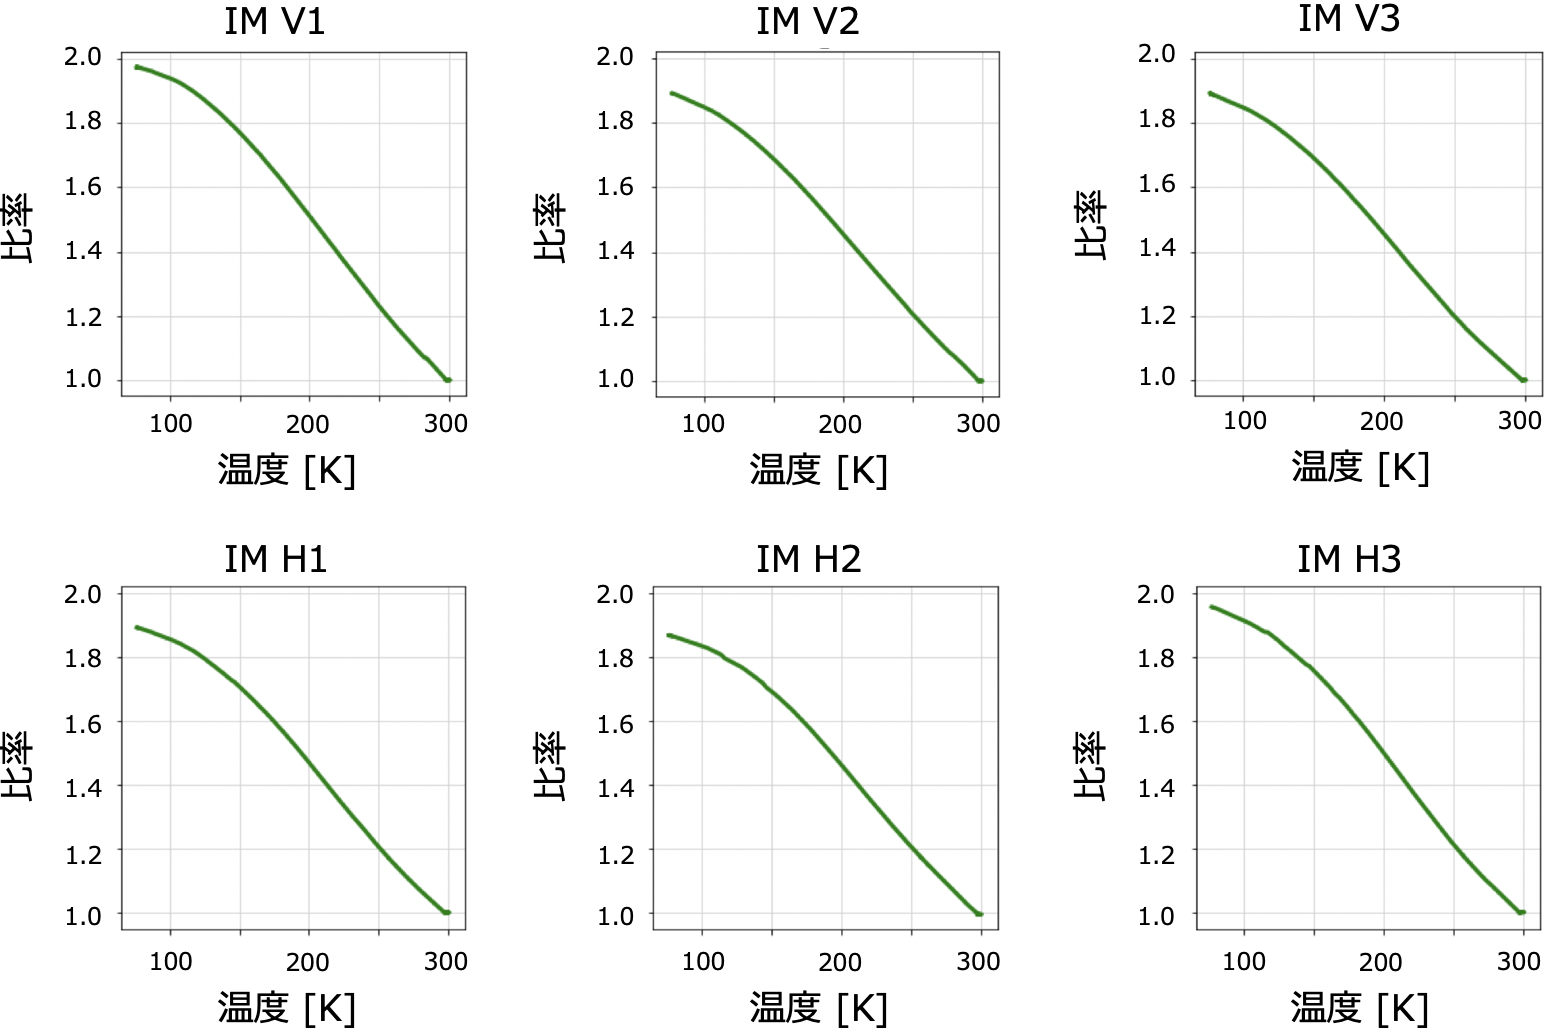
\includegraphics[width=160mm]{fig5_3.png}
\caption[フォトセンサの出力(ETMX IM)の変化]{フォトセンサの出力(ETMX MN)の変化}
\label{fig5.3}
\end{center}
\end{figure}
\begin{figure}[H]
\begin{center}
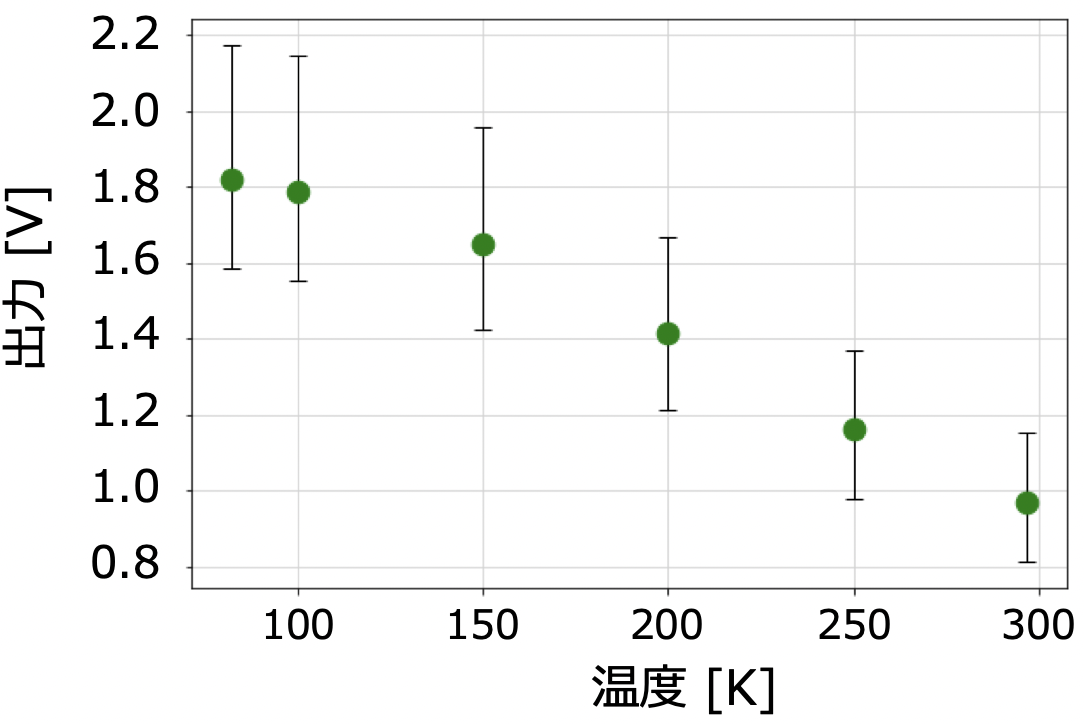
\includegraphics[width=140mm]{fig5_4.png}
\caption[温度ごとのフォトセンサの出力]{温度ごとのフォトセンサの出力の平均. エラーバーはそれぞれ出力の最小値, 最大値を表している.}
\label{fig5.4}
\end{center}
\end{figure}
\begin{table}[H]
 \centering
  \begin{tabular}{|c||c|c|c|c|}
   \hline
    温度& 平均値 & 標準偏差 & 最大最小の差  \\
   \hline
   297 K & 0.9662 V & 0.1021 V & 0.3389 V\\
   \hline
   250 K    &  1.163 V & 0.1219 V & 0.3907 V\\
   \hline
   200 K    & 1.414 V & 0.1494 V & 0.4559 V\\
   \hline
   150 K    & 1.648 V & 0.1775 V & 0.5310 V\\
   \hline
    100 K    & 1.789 V & 0.1906 V & 0.5904 V\\
   \hline
    82 K    & 1.822 V & 0.2044 V & 0.5915 V\\
   \hline
  \end{tabular}
 \caption[フォトセンサの出力の平均値およびばらつき]{フォトセンサの出力の平均値およびばらつき}
 \label{table5.1}
\end{table}
また, 図\ref{fig5.4}に示したのは各温度における12個のフォトセンサの出力の平均である.  なお, エラーバーはそれぞれ出力の最小値, 最大値を表している. さらに, 各温度における出力の平均値および標準偏差は表\ref{table5.1}の通りであり, これらより低温にすると出力のばらつきが大きくなるのが分かる.
\subsubsection{考察}
\vskip3mm
\cite{47}によると, センサの個体差が50\%以下であるという要求がある. これはキャリブレーションファクターの大きさが50\%以上変化すると, センサとターゲットの距離が$\pm 1$ cmという線形応答範囲にあるかどうか分からなくなるからである. 本研究において, 実際にKAGRAへインストールして冷却された状態で出力のばらつきを測定した結果, センサの個体差は82 Kにおいても平均値に対して32\%であり, 50\%以下という要求を満たすことが分かった. しかし, 低温にすると出力のばらつきは大きくなっており, 冷却が進むにつれてセンサの個体差がさらに広がる恐れがある. したがって, 今後さらに冷却する場合, フォトセンサの出力のばらつきに注意する必要がある.\\
\quad 補遺\ref{補遺C}に示したように, 反射型フォトセンサの出力はLEDのビームプロファイルに大きく影響を受ける. よってフォトセンサの出力のばらつきの原因としてLEDのビームプロファイルの違いが挙げられる. しかし, 低温でそのばらつきが大きくなる理由は説明できない. KAGRAの反射型フォトセンサに用いられるLEDの発光効率の個体差および温度との関係については, 今後調査する必要がある.

\subsection{共振周波数・伝達関数}
\subsubsection{測定結果}
\vskip3mm
MN段の各自由度方向 (L, P, Y) に励起信号を入れて振動させ, フォトセンサの出力で読み取ったMN段の各方向の動きまでの伝達関数を測定した. その結果を図\ref{fig5.5}, \ref{fig5.6}, \ref{fig5.7}に示す. これらより, 低温にすると共振周波数が数\%高くなっているのが分かる.
\begin{figure}[H]
\begin{center}
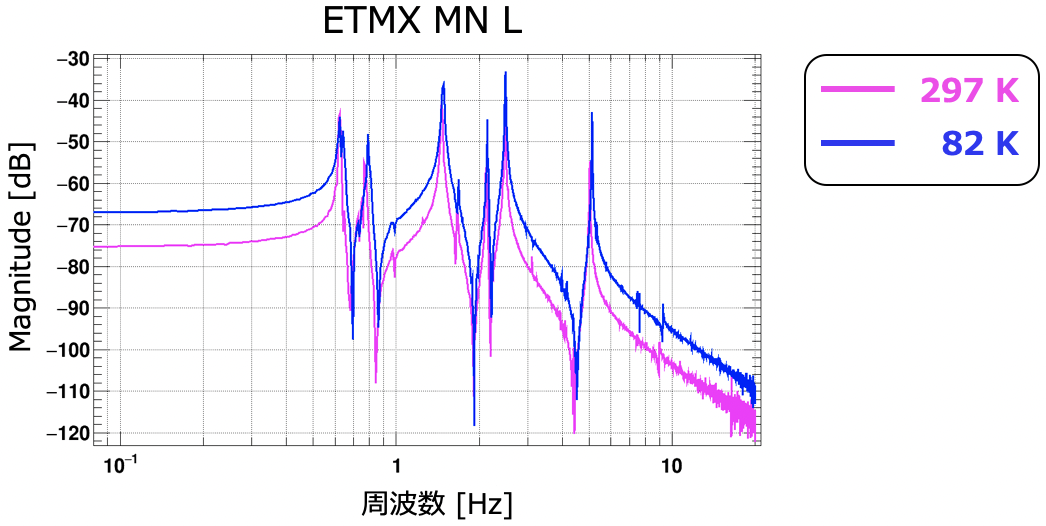
\includegraphics[width=150mm]{fig5_5.png}
\caption[室温と低温での伝達関数の比較 (L)]{室温と低温での伝達関数の比較(ETMXのMNのL). ピンク, 青の線がそれぞれ室温 (297 K) , 低温 (82 K) における伝達関数を示している.  }
\label{fig5.5}
\end{center}
\end{figure}
\begin{figure}[H]
\begin{center}
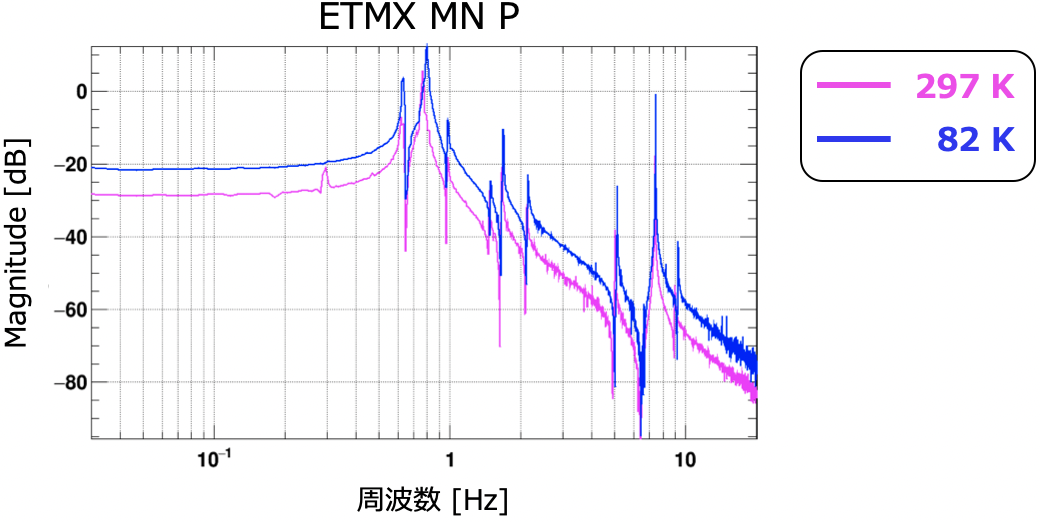
\includegraphics[width=150mm]{fig5_6.png}
\caption[室温と低温での伝達関数の比較 (P)]{室温と低温での伝達関数の比較(ETMXのMNのP). ピンク, 青の線がそれぞれ室温 (297 K) , 低温 (82 K) における伝達関数を示している.  }
\label{fig5.6}
\end{center}
\end{figure}
\begin{figure}[H]
\begin{center}
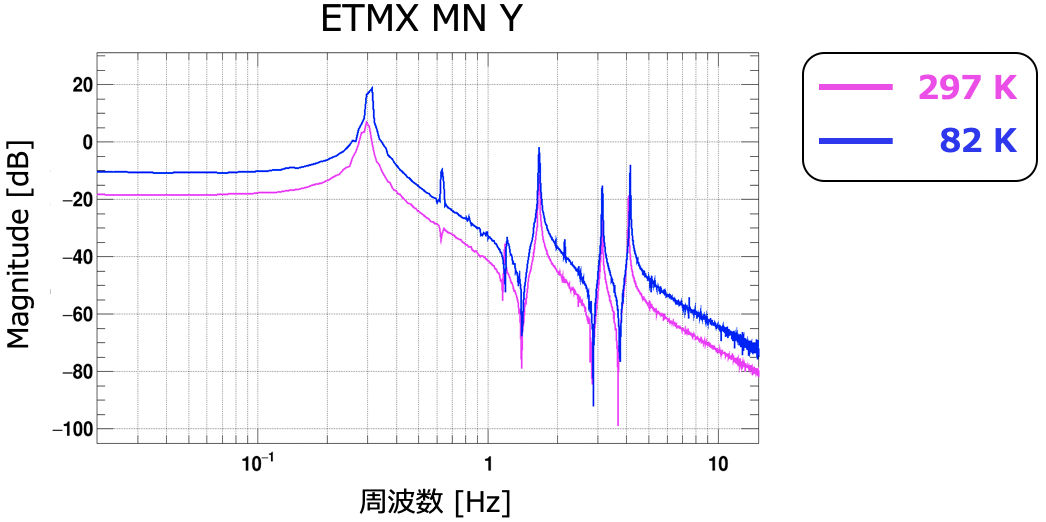
\includegraphics[width=150mm]{fig5_7.png}
\caption[室温と低温での伝達関数の比較 (Y)]{室温と低温での伝達関数の比較(ETMXのMNのY). ピンク, 青の線がそれぞれ室温 (297 K) , 低温 (82 K) における伝達関数を示している. }
\label{fig5.7}
\end{center}
\end{figure}
\begin{table}[H]
 \centering
  \begin{tabular}{|c||c|c|c|c|}
   \hline
    \diagbox{温度}{Mode}& 1 & 2 & 3 & 4 \\
   \hline
   297 K & 0.63 Hz & 1.46 Hz & 2.12 Hz & 2.47 Hz \\
   \hline
   82 K    & 0.63 Hz & 1.48 Hz & 2.13 Hz & 2.48 Hz \\
   \hline
  \end{tabular}
 \caption[共振周波数 (ETMX MN L)]{共振周波数 (ETMX MN L)}
\end{table}
\begin{table}[H]
 \centering
  \begin{tabular}{|c||c|c|c|c|}
   \hline
    \diagbox{温度}{Mode}& 1 & 2  \\
   \hline
   297 K & 0.76 Hz & 7.42 Hz  \\
   \hline
   82 K    & 0.80 Hz & 7.46 Hz \\
   \hline
  \end{tabular}
 \caption[共振周波数 (ETMX MN P)]{共振周波数 (ETMX MN P)}
\end{table}
\begin{table}[H]
 \centering
  \begin{tabular}{|c||c|c|c|c|}
   \hline
    \diagbox{温度}{Mode}& 1 & 2 & 3 & 4 \\
   \hline
   297 K & 0.29 Hz & 1.66 Hz & 3.13 Hz & 4.08 Hz \\
   \hline
   82 K    & 0.31 Hz & 1.67 Hz & 3.14 Hz & 4.16Hz \\
   \hline
  \end{tabular}
 \caption[共振周波数 (ETMX MN Y)]{共振周波数 (ETMX MN Y)}
\end{table} 
\subsubsection{考察}
\vskip3mm
一般に, 低温にするとヤング率が上昇することで共振周波数が増加すると考えられ, 予想通りの結果が得られたといえる. \\
\quad また, 励起信号からMNの動きまでの伝達関数のゲインが上がっているが, これはフォトセンサの出力が増加したことに由来する. フォトセンサの出力を各方向の変異に換算しているが, 冷却に伴いセンサの出力が増加した分を校正していないため伝達関数のゲインが上がっているのである.
\subsection{機械的Q値}
%機械的Q値(以下Q値と記述する)は共振の鋭さを表すパラメータであり, この値が大きいほど振動のエネルギーは共振のピークに押し込められる. これは共振周波数以外でのエネルギーが下がるということを意味しており, ゆえにQ値は熱雑音低減のために重要な値である. 
\subsubsection{測定方法}
\vskip3mm
Q値は伝達関数から求めることができる. 例えば減衰を含む調和振動子の運動方程式は
\begin{equation}
m\ddot{x}+m\omega_0^2x=f(t),
\label{eq5.1}
\end{equation}
と書けるが, これをFourier変換した上で散逸を表す項$\phi(\omega)$を付け加えると
\begin{equation}
-m\omega^2\tilde{x}+m\omega_0^2\left[1+i\phi(\omega)\right]\tilde{x}=\tilde{f},
\end{equation}
となる. なお, この$\phi(\omega)$を用いると位置および復元力は周波数領域において
\begin{equation}
\tilde{F}=-m\omega_0^2\left[1+i\phi(\omega)\right]\tilde{x},
\end{equation}
と書ける. つまり, 復元力の位相は位置の位相に対して$\phi$遅れる. ここで, 復元力が1周期の間にする仕事(復元力による仕事率$F\dot{x}$を1周期で積分したもの)を計算し, 系の全エネルギーで規格化すると$-2\pi\phi$となる. これが散逸したエネルギーであり, $\phi(\omega)$が散逸を示す項であることが分かる. \\
\quad ここで
\begin{equation}
\phi(\omega_0)=\frac{1}{Q},
\end{equation}
となる$Q$が機械的Q値である.\\
\quad この調和振動子の伝達関数の絶対値の2乗は
\begin{equation}
\left|H(\omega)\right|^2=\frac{1}{m^2\left\{(\omega^2-\omega_0^2)^2+w_0^4\phi^2(\omega)\right\}^2}.
\end{equation}
これは$\omega=\omega_0$のときにピークを持つが, その半値幅を$\Delta\omega_0$とすると
\begin{equation}
\left|H\left(\omega_0\pm\frac{\Delta\omega_0}{2}\right)\right|^2=\frac{\left|H(\omega_0)\right|^2}{2},
\end{equation}
でありピークの幅が小さいときは$\Delta\omega_0\ll\omega_0$であり, さらに$\phi(\omega)=\phi(\omega_0)=1/Q$と書けるので
\begin{equation}
\Delta\omega_0=\frac{\omega_0}{Q},
\label{eq5.7}
\end{equation}
となる. 式(\ref{eq5.7})から分かるように, Q値が低いほど半値幅$\Delta\omega_0$は大きくなる. よって伝達関数のピークの半値幅からQ値を求めるこの方法は, Q値が低い場合は有効である. \\
\quad しかし, 本研究における懸架系のQ値はある程度大きいため, 懸架系に外力を加えた時の減衰時間から求める手法をとる. 先ほどの調和振動子の式(\ref{eq5.1})において外力項を
\begin{equation}
f(t) = 
    \begin{cases}
        {A{\rm exp}(i\omega_0t) \quad (t<0)}\\
        {0 \quad\quad\quad \quad\quad\,\, (t>0)}
    \end{cases},
\end{equation}
とする. このとき, 運動方程式をFourier変換して$\tilde{x}$について解いた上で逆Fourier変換すると
\begin{equation}
x(t)\propto {\rm exp}\left(-\frac{\omega_0t}{2Q}\right).
\end{equation}
これより, 共振状態に励起した後で励起信号を切り, 振動の減衰時間を測定することでQ値を求めることができる. すなわち, 減衰の時定数を$\tau$としたとき
\begin{equation}
x(t)\propto {\rm exp}\left(-\frac{t}{\tau}\right),
\label{eq5.10}
\end{equation}
であるから$f_0=\frac{\omega_0}{2\pi}$を用いて
\begin{equation}
\tau=\frac{2Q}{\omega_0}=\frac{2Q}{2\pi f_0}=\frac{Q}{\pi f_0},
\end{equation}
となり, 
\begin{equation}
Q=\pi f_0\tau,
\label{eq5.12}
\end{equation}
と計算できる. \\
\quad 式(\ref{eq5.12})から分かる通りQ値が高いほど減衰時間が長く, フィッティングの精度が上がるため, 本研究の場合のような高いQ値の測定にはこの方法を用いる. \\
\quad 実際には, MN段に対応する共振周波数に等しい周波数の励起信号を入れた後でその励起を止め, 振動が減衰する時間を測定する. このとき, 減衰の様子は図\ref{fig5.8}に示す通りであり, Q値が大きいため振動が十分減衰するのに時間がかかるのが分かる. 減衰時間は式(\ref{eq5.10})で示したように減衰曲線の包絡線を指数関数でフィッティングすれば良い. 
%\footnote[100]{このままでは外乱があった際に干渉計が再ロックするまで長時間待たないといけないため, 次章に示すダンピング制御を行う. }
\begin{figure}[H]
\begin{center}
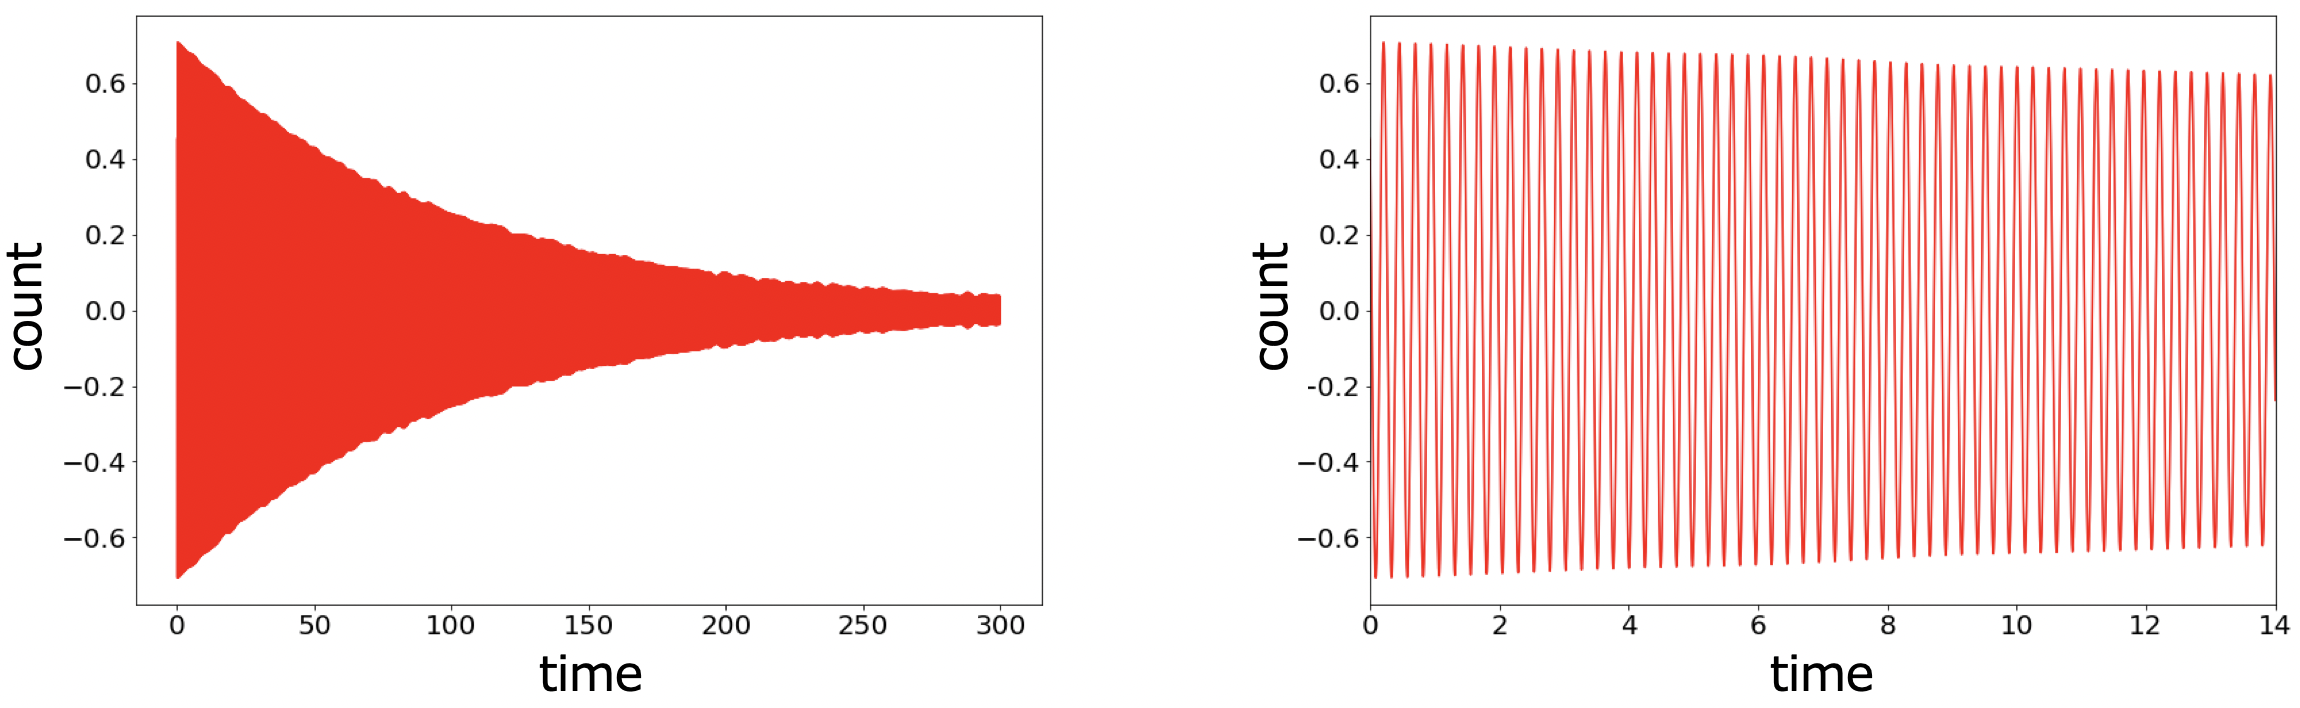
\includegraphics[width=170mm]{fig5_100.png}
\caption[励起信号を切った後の減衰の様子]{左図はETMXのMN段にY方向の励起信号 (4.08 Hz) を入れて共振状態にした後に励起信号を切ったとき, 振動が減衰する様子を示したものである. Q値が大きいため振動が十分減衰するまでは時間がかかる(右図は初めの約15秒間を拡大したものである). }
\label{fig5.8}
\end{center}
\end{figure}
\subsubsection{測定結果}
\vskip3mm
297 Kと82 KにおいてETMXのMNでQ値を測定した結果, L, P, Yのそれぞれの自由度に対する結果は表\ref{table5.5}, \ref{table5.6}, \ref{table5.7}のようになった. また, これを図示すると図\ref{fig5.9}のようになる. 
\begin{table}[H]
 \centering
  \begin{tabular}{|c||c|c|c|c|}
   \hline
    \diagbox{温度}{Mode}& 1 & 2 & 3 & 4 \\
   \hline 
   297 K & 1760.8 & 1251.7 & 2981.5 & 3160.4 \\
   \hline
   82 K    & 1504.0 & 1228.6 & 4245.6 & 1996.1 \\
   \hline
  \end{tabular}
 \caption[Q値 (ETMX MN L)]{Q値 (ETMX MN L)}
 \label{table5.5}
\end{table}
\begin{table}[H]
 \centering
  \begin{tabular}{|c||c|c|}
   \hline
    \diagbox{温度}{Mode}& 1 & 2  \\
   \hline 
   297 K & 435.47 & 3460.3 \\
   \hline
   82 K    & 440.38 & 9548.2 \\
   \hline
  \end{tabular}
 \caption[Q値 (ETMX MN P)]{Q値 (ETMX MN P)}
  \label{table5.6}
\end{table}
\begin{table}[H]
 \centering
  \begin{tabular}{|c||c|c|c|c|}
   \hline
    \diagbox{温度}{Mode}& 1 & 2 & 3 & 4 \\
   \hline
   297 K & 233.94 & 2603.5 & 4703.8 & 1245.2 \\
   \hline
   82 K    & 131.86 & 1789.9 & 5291.8 & 2287.2 \\
   \hline
  \end{tabular}
 \caption[Q値 (ETMX MN Y)]{Q値 (ETMX MN Y)}
  \label{table5.7}
\end{table}
\begin{figure}[H]
\begin{center}
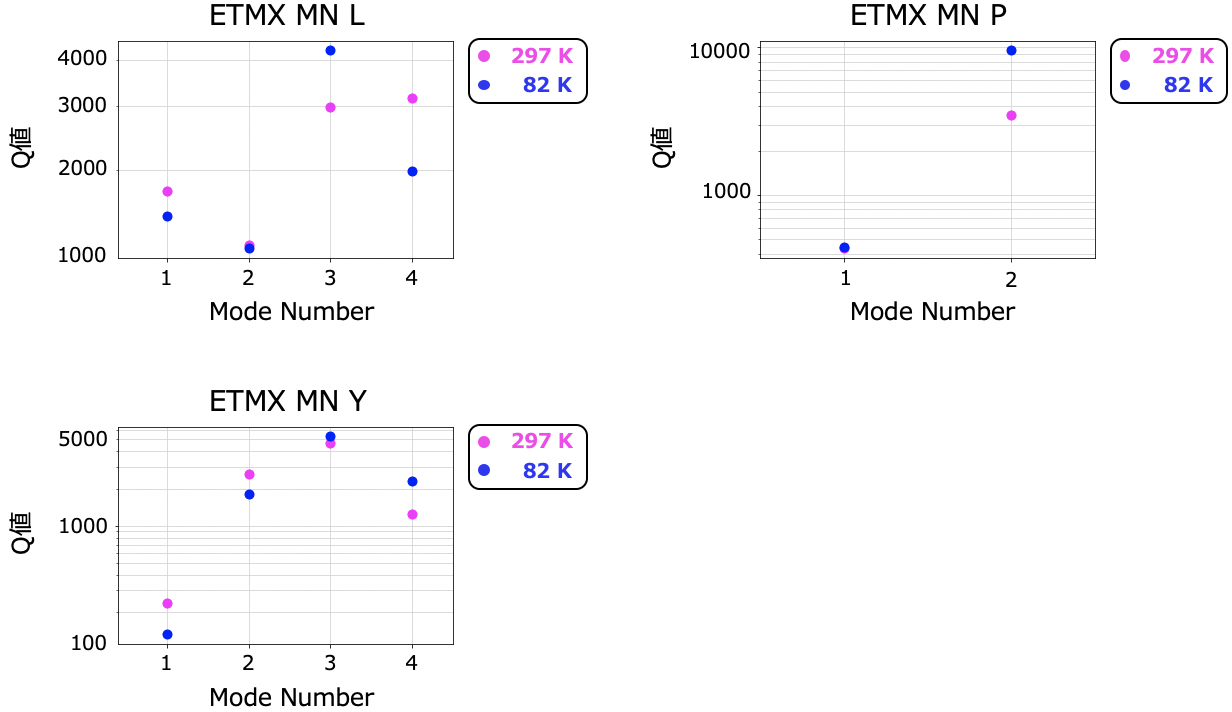
\includegraphics[width=170mm]{fig5_101.png}
\caption[室温と低温でのQ値の比較]{室温と低温でのQ値の比較(ETMXのMNのL,  P, Y). ピンク, 青の点がそれぞれ室温 (297 K) , 低温 (82 K) におけるQ値を示している. サファイアが低温においてQ値が高いという性質を持つため, 一般には, サファイアファイバーの影響が大きいモードでは低温にするとQ値が大きくなる. }
 \label{fig5.9}
\end{center}
\end{figure}
\subsubsection{考察}
\vskip3mm
%{\color{red}「サファイアが低温においてQ値が高いという性質を持つため, 一般には, サファイアファイバーの影響が大きいモードでは低温にするとQ値が大きくなる. 」という内容を書く. モードの説明・図示しながら. }
図5.7を見ると, Lの3つめのモード, Pの2つめのモード, Yの4つめのモードでは低温にした時にQ値が増加している.  これは2.2.4.2で述べたように, 低温で高いQ値を示すサファイアファイバーの影響を大きく受けるからであると考えられる. 実際, \cite{eigen}にまとめられたType-A suspensionの固有モードのリストによると, これらのモードはサファイアファイバー(低温懸架装置の下部)の影響を大きく受けるモードとなっており, 本研究で得られた結果と合致している.\\
\quad また, ダンピング制御に変更の必要性があるかどうかは第\ref{第6章}章に示す.
